\documentclass[MAIN.tex]{subfiles}
\begin{document}
	\chapter{Introduction to Method Comparison Studies}
	
	
	
	\section{Agreement}
	\begin{itemize}
		\item The FDA define precision as the \textit{closeness of agreement} (degree of
		scatter) between a series of measurements obtained from multiple
		sampling of the same homogeneous sample under prescribed
		conditions. 
		\item \textbf{Barnhart} describes precision as being further
		subdivided as either within-run, intra-batch precision or
		repeatability (which assesses precision during a single analytical
		run), or between-run, inter-batch precision or repeatability
		(which measures precision over time).
	\end{itemize}
	
	
	
	\section{Purposes of MCS}
	
	The  question being answered is not always clear, but is usually epxressed as an attempt to quantify the agreement
	between two methods (Bland and Altman 1995)
	
	Some lack of agreement between different methods of measurement is inevitable. What matters is the amount by which they
	disagree. we want to know by how much the new method is likely to differ from the old, so that it is not enough to cause
	problems in the mathematical interpretation we can preplace the old method by the new, or even use the two interchangably.
	
	
	It often happens that the same physical and chemical property can be measured in different ways. For example, one can determine
	For example, one can determine sodium in serum by flame atomic emission spectroscopy or by isotops dilution mass spectroscopy. The question arises as to whcih methd is better (Mandel 1991)
	
	In areas of inter-laboratory quality control, method comparisons, assay validations and individual bio-equivalence, etc, the agree between observations and target (reference) value is
	of interest (lin 2002)
	
	The purpose of comparing two methods of measurement of a continuous biological variable is to uncover systematic differences, not to point to
	similarities. (ludbrook 1997)
	
	In the pharmaceutical industry, measurement methods that measure the quantity of prdocuts are regulated. The FDA (U.S. Food and
	Drug Administration) requires that the manufacturer show equivalency prior to approving the new or alternatice method in quality control (Tan \& Inglewicz ,1999)
	
	
	\section{Indications on how to deal with outliers in Bland Altman plots}
	
	We wish to determine how outliers should be treated in a Bland
	Altman Plot
	
	In their 1983 paper they merely state that the plot can be used to
	'spot outliers'.
	
	In  their 1986 paper, Bland and Altman give an example of an
	outlier. They state that it could be omitted in practice, but make
	no further comments on the matter.
	\\
	In Bland and Altmans 1999 paper, we get the clearest indication of
	what Bland and Altman suggest on how to react to the presence of
	outliers. Their recommendation is to recalculate the limits
	without them, in order to test the difference with the calculation
	where outliers are retained.\\
	
	The span has reduced from 77 to 59 mmHg, a noticeable but not
	particularly large reduction.
	\\
	However, they do not recommend removing outliers. Furthermore,
	they say:
	\\
	We usually find that this method of analysis is not too sensitive
	to one or two large outlying differences.
	\\
	We ask if this would be so in all cases. Given that the limits of
	agreement may or may not be disregarded, depending on their
	perceived suitability, we examine whether it would possible that
	the deletion of an outlier may lead to a calculation of limits of
	agreement that are usable in all cases?
	\\
	Should an Outlying Observation be omitted from a data set? In
	general, this is not considered prudent.
	\\
	Also, it may be required that the outliers are worthy of
	particular attention themselves.
	\\
	Classifying outliers and recalculating We opted to examine this
	matter in more detail. The following points have to be considered
	\\how to suitably identify an outlier (in a generalized sense)
	\\Would a recalculation of the limits of agreement generally
	results in  a compacted range between the upper and lower limits
	of agreement?
	\subsection{Agreement} Bland and Altman (1986) define Perfect
	agreement as 'The case where all of the pairs of rater data lie
	along the line of equality'. The Line of Equality is defined as
	the 45 degree line passing through the origin, or X=Y on a XY
	plane.
	
	
	\section{Roy's Approach}
	
	For the purposes of comparing two methods of measurement, \citet{ARoy2009} presents a methodology utilizing linear mixed effects model. This methodology provides for the formal testing of inter-method bias, between-subject variability and within-subject variability of two methods. 
	
	\citet{ARoy2009} uses an approach based on linear mixed effects (LME) models for the purpose of comparing the agreement between two methods of measurement, where replicate measurements on items (often individuals) by both methods are available. Three tests of hypothesis appropriate are provided for evaluating the agreement between the two methods of measurement under this sampling scheme. 
	
	Importantly \citet{ARoy2009} further proposes a series of three tests on the variance components of an LME model, which allow decisions on the second and third of Roy's criteria. For these tests, four candidate LME models are constructed. 
	
	\citet{ARoy2009} proposes the use of LME models to perform a test on two methods of agreement to comparing the agreement between two methods of measurement, where replicate measurements on items (often individuals) by both methods are available, determining whether they can be used
	interchangeably. The methodology proposed by \citet{ARoy2009} is largely based on \citet{hamlett}, which in turn follows on from \citet{lam}.
	
	\citet{ARoy2009} proposes a novel method using the LME model with Kronecker product covariance structure in a doubly multivariate set-up to assess the agreement between a new method and an established method with unbalanced data and with unequal replications for different subjects. By doubly multivariate set up, Roy means that the information on each patient or item is multivariate at two levels, the number of methods and number of replicated measurements. Further to \citet{lam}, it is assumed that the replicates are linked over time. However it is easy to modify to the unlinked case.
	
	
	The well-known ``Limits of Agreement", as developed by \citet{BA86} are not referred to directly, but are easily computable using the framework proposed by \citet{ARoy2009}. Further discussion will be provided in due course.	
	
	
	
	
	
	%Two methods of measurement can be said to be in agreement if there is no significant difference between in three key respects. 
	%
	%Firstly, there is no inter-method bias between the two methods, i.e. there is no persistent tendency for one method to give higher values than the other.
	%
	%Secondly, both methods of measurement have the same  within-subject variability. In such a case the variance of the replicate measurements would consistent for both methods.
	%Lastly, the methods have equal between-subject variability.  Put simply, for the mean measurements for each case, the variances of the mean measurements from both methods are equal.
	
	Further to this, \citet{ARoy2009} demonstrates an suite of tests that can be used to determine how well two methods of measurement, in the presence of repeated measures, agree with each other.
	
	\begin{itemize}\itemsep0.5cm
		\item No Significant inter-method bias
		\item No difference in the between-subject variabilities of the two methods
		\item No difference in the within-subject variabilities of the two methods
	\end{itemize}
	
	The formulation presented above usefully facilitates a series of
	significance tests that advise as to how well the two methods
	agree. These tests are as follows:
	\begin{itemize}
		\item A formal test for the equality of between-item variances,
		\item A formal test for the equality of within-item variances,
		\item A formal test for the equality of overall variances.
	\end{itemize}
	These tests are complemented by the ability to consider the inter-method bias and the overall correlation coefficient. Two methods can be considered to be in agreement if criteria based upon these methodologies are met. Additionally Roy makes reference to the overall correlation coefficient of the two methods, which is determinable from variance estimates. Other important aspects of the method comparison study are consequent. The limits of agreement are computed using the results of the reference model.
	
	Differences in between-subject variabilities of the two methods arise when one method is yielding average response levels for individuals than are more variable than the average response levels for the same sample of individuals taken by the other method.  Differences in within-subject variabilities of the two methods arise when one method is yielding responses for an individual than are more variable than the responses for this same individual taken by the other method. The two methods of measurement can be considered to agree, and subsequently can be used interchangeably, if all three null hypotheses are true.	
	
	
	\subsection{LME Model Specification}
	
	Let $y_{mir} $ denote the $r$th replicate measurement on the $i$th item by the $m$th method, where $m=1,2,$ $i=1,\ldots,N,$ and $r = 1,\ldots,n_i.$ When the design is balanced and there is no ambiguity we can set $n_i=n.$ The LME model underpinning Roy's approach can be written
	\begin{equation}\label{Roy-model}
		y_{mir} = \beta_{0} + \beta_{m} + b_{mi} + \epsilon_{mir}.
	\end{equation}
	
	Here $\beta_0$ and $\beta_m$ are fixed-effect terms representing, respectively, a model intercept and an overall effect for method $m.$ 
	
	The $b_{1i}$ and $b_{2i}$ terms represent random effect parameters corresponding to the two methods, having $\mathrm{E}(b_{mi})=0$ with $\mathrm{Var}(b_{mi})=g^2_m$ and $\mathrm{Cov}(b_{mi}, b_{m^\prime i})=d_{12}.$ The random error term for each response is denoted $\epsilon_{mir}$ having $\mathrm{E}(\epsilon_{mir})=0$, $\mathrm{Var}(\epsilon_{mir})=\sigma^2_m$, $\mathrm{Cov}(b_{mir}, b_{m^\prime ir})=\sigma_{12}$, $\mathrm{Cov}(\epsilon_{mir}, \epsilon_{mir^\prime})= 0$ and $\mathrm{Cov}(\epsilon_{mir}, \epsilon_{m^\prime ir^\prime})= 0.$
	
	
	When two methods of measurement are in agreement, there is no significant differences between $\beta_1$ and $\beta_2,$ $g^2_1 $ and$ g^2_2$, and $\sigma^2_1 $ and$ \sigma^2_2$.
	Here $\beta_0$ and $\beta_m$ are fixed-effect terms representing, respectively, a model intercept and an overall effect for method $m.$ 
	
	The model can be reparameterized by gathering the $\beta$ terms together into (fixed effect) intercept terms $\alpha_m=\beta_0+\beta_m.$ The $b_{1i}$ and $b_{2i}$ terms are correlated random effect parameters having $\mathrm{E}(b_{mi})=0$ with $\mathrm{Var}(b_{mi})=g^2_m$ and $\mathrm{Cov}(b_{1i}, b_{2 i})=d_{12}.$ 
	
	The random error term for each response is denoted $\epsilon_{mir}$ having $\mathrm{E}(\epsilon_{mir})=0$, $\mathrm{Var}(\epsilon_{mir})=\sigma^2_m$, $\mathrm{Cov}(\epsilon_{1ir}, \epsilon_{2 ir})=\sigma_{12}$, $\mathrm{Cov}(\epsilon_{mir}, \epsilon_{mir^\prime})= 0$ and $\mathrm{Cov}(\epsilon_{1ir}, \epsilon_{2 ir^\prime})= 0.$ Two methods of measurement are in complete agreement if the null hypotheses $\mathrm{H}_1\colon \alpha_1 = \alpha_2$ and $\mathrm{H}_2\colon \sigma^2_1 = \sigma^2_2 $ and $\mathrm{H}_3\colon g^2_1= g^2_2$ hold simultaneously. \citet{ARoy2009} uses a Bonferroni correction to control the familywise error rate for tests of $\{\mathrm{H}_1, \mathrm{H}_2, \mathrm{H}_3\}$ and account for difficulties arising due to multiple testing. 
	\subsection{Variance Covariance Matrices }
	
	Under Roy's model, random effects are defined using a bivariate normal distribution. Consequently, the variance-covariance structures can be described using $2 \times 2$  matrices. A discussion of the various structures a variance-covariance matrix can be specified under is required before progressing. The following structures are relevant: the identity structure, the compound symmetric structure and the symmetric structure.
	
	The differences in the models are specifically in how the the $D$ and $\Lambda$ matrices are constructed, using either an unstructured form or a compound symmetry form. To illustrate these differences, consider a generic matrix $A$,
	
	\[
	\boldsymbol{A} = \left( \begin{array}{cc}
	a_{11} & a_{12}  \\
	a_{21} & a_{22}  \\
	\end{array}\right).
	\]
	
	A symmetric matrix allows the diagonal terms $a_{11}$ and $a_{22}$ to differ. The compound symmetry structure requires that both of these terms be equal, i.e $a_{11} = a_{22}$.
	
	
	The identity structure is simply an abstraction of the identity matrix. The compound symmetric structure and symmetric structure can be described with reference to the following matrix (here in the context of the overall covariance Block-$\boldsymbol{\Omega}_i$, but equally applicable to the component variabilities $\boldsymbol{D}$ and $\boldsymbol{\Sigma}$);
	
	\[\left( \begin{array}{cc}
	\omega^2_1  & \omega_{12} \\
	\omega_{12} & \omega^2_2 \\
	\end{array}\right) \]
	
	Symmetric structure requires the equality of all the diagonal terms, hence $\omega^2_1 = \omega^2_2$. Conversely compound symmetry make no such constraint on the diagonal elements. Under the identity structure, $\omega_{12} = 0$.
	A comparison of a model fitted using symmetric structure with that of a model fitted using the compound symmetric structure is equivalent to a test of the equality of variance.
	
	
	%In the presented example, it is shown that Roy's LOAs are lower than those of (\ref{BXC-model}), when covariance between methods is present.
	
	
	
	\subsubsection{Independence}
	
	As though analyzed using between subjects analysis.
	\[
	\left(
	\begin{array}{c c c}
	\psi^2 & 0 & 0   \\
	0 & \psi^2 & 0   \\
	0 & 0 & \psi^2   \\
	\end{array}%
	\right)
	\]
	
	
	
	\subsubsection{Compound Symmetry}
	
	Assumes that the variance-covariance structure has a single variance (represented by $\psi^2$)
	for all 3 of the time points and a single covariance (represented by $\psi_{ij}$) for each of the pairs of trials.
	
	\[
	\left(%
	\begin{array}{c c c}
	\psi^2 &  \psi_{12} & \psi_{13}   \\
	\psi_{21} & \psi^2 & \psi_{23}   \\
	\psi_{31} & \psi_{32} & \psi^2   \\
	\end{array}%
	\right)
	\]
	
	
	%\subsubsection{Unstructured}
	%
	%Assumes that each variance and covariance is unique.
	%Each trial has its own variance (e.g. s12 is the variance of trial 1)
	%and each pair of trials has its own covariance (e.g. s21 is the covariance of trial 1 and trial2).
	%This structure is illustrated by the half matrix below.
	%
	%
	%
	%\subsubsection{Autoregressive}
	%
	%Another common covariance structure which is frequently observed
	%in repeated measures data is an autoregressive structure,
	%which recognizes that observations which are more proximate
	%are more correlated than measures that are more distant.
	%
	%
	
	
	
	
	
	
	%-----------------------------------------------------------------------------------------------------%
	
	
	
	
	
	\subsection{Model Terms (Roy 2009)}
	\begin{itemize}
		\item Let $y_{mir}$ be the response of method $m$ on the $i$th subject
		at the $r-$th replicate.
		\item Let $\boldsymbol{y}_{ir}$ be the $2 \times 1$ vector of measurements
		corresponding to the $i-$th subject at the $r-$th replicate.
		\item Let $\boldsymbol{y}_{i}$ be the $R_i \times 1$ vector of
		measurements corresponding to the $i-$th subject, where $R_i$ is number of replicate measurements taken on item $i$.
		\item Let $\alpha_mi$ be the fixed effect parameter for method for subject $i$.
		\item Formally ARoy2009 uses a separate fixed effect parameter to describe the true value $\mu_i$, but later combines it with the other fixed effects when implementing the model.
		\item Let $u_{1i}$ and $u_{2i}$ be the random effects corresponding to methods for item $i$.
		
		\item $\boldsymbol{\epsilon}_{i}$ is a $n_{i}$-dimensional vector
		comprised of residual components. For the blood pressure data $n_{i} = 85$.
		
		\item $\boldsymbol{\beta}$ is the solutions of the means of the two methods. In the LME output, the bias ad corresponding
		t-value and p-values are presented. This is relevant to ARoy2009's first test.\end{itemize}
	
	
	
	\subsection{Model Terms (Roy 2009)}
	It is important to note the following characteristics of this model.
	
	Let the number of replicate measurements on each item $i$ for both methods be $n_i$, hence $2 \times n_i$ responses. However, it is assumed that there may be a different number of replicates made for different items. Let the maximum number of replicates be $p$. An item will have up to $2p$ measurements, i.e. $\max(n_{i}) = 2p$.
	
	% \item $\boldsymbol{y}_i$ is the $2n_i \times 1$ response vector for measurements on the $i-$th item.
	% \item $\boldsymbol{X}_i$ is the $2n_i \times  3$ model matrix for the fixed effects for observations on item $i$.
	% \item $\boldsymbol{\beta}$ is the $3 \times  1$ vector of fixed-effect coefficients, one for the true value for item $i$, and one effect each for both methods.
	
	Later on $\boldsymbol{X}_i$ will be reduced to a $2 \times 1$ matrix, to allow estimation of terms. This is due to a shortage of rank. The fixed effects vector can be modified accordingly.
	
	$\boldsymbol{Z}_i$ is the $2n_i \times  2$ model matrix for the random effects for measurement methods on item $i$.\\
	\bigskip
	
	$\boldsymbol{b}_i$ is the $2 \times  1$ vector of random-effect coefficients on item $i$, one for each method.
	
	$\boldsymbol{\epsilon}$  is the $2n_i \times  1$ vector of residuals for measurements on item $i$.\\
	\bigskip
	
	$\boldsymbol{G}$ is the $2 \times  2$ covariance matrix for the random effects.
	
	$\boldsymbol{R}_i$ is the $2n_i \times  2n_i$ covariance matrix for the residuals on item $i$.
	
	The expected value is given as $\mbox{E}(\boldsymbol{y}_i) = \boldsymbol{X}_i\boldsymbol{\beta}.$ \citep{hamlett}\\
	\bigskip
	
	The variance of the response vector is given by $\mbox{Var}(\boldsymbol{y}_i)  = \boldsymbol{Z}_i \boldsymbol{G} \boldsymbol{Z}_i^{\prime} + \boldsymbol{R}_i$ \citep{hamlett}.
	
	
	
	$\boldsymbol{b}_{i}$ is a $m-$dimensional vector comprised of
	the random effects.
	\begin{equation}
		\boldsymbol{b}_{i} = \left( \begin{array}{c}
			b_{1i} \\
			b_{21}  \\
		\end{array}\right)
	\end{equation}
	
	
	$\boldsymbol{V}$ represents the correlation matrix of the replicated measurements on a given method.
	$\boldsymbol{\Sigma}$ is the within-subject VC matrix.\\
	\bigskip
	
	
	$\boldsymbol{V}$ and $\boldsymbol{\Sigma}$ are positive
	definite matrices. The dimensions of $\boldsymbol{V}$ and
	$\boldsymbol{\Sigma}$ are $3 \times 3 ( = p \times p )$ and $ 2 \times
	2 (= k \times k)$.\\
	\bigskip
	
	
	It is assumed that $\boldsymbol{V}$ is the same for both methods and $\boldsymbol{\Sigma}$ is
	the same for all replications.\\
	\bigskip
	
	$\boldsymbol{V} \bigotimes \boldsymbol{\Sigma}$ creates a $ 6 \times 6 ( = kp \times
	kp)$ matrix.
	$\boldsymbol{R}_{i}$ is a sub-matrix of this.\\
	\bigskip
	
	% Complete paragraph by specifying variances and covariances for epsilons.
	% I thing that these are your sigmas?
	% Also, state equality of the parameters in this model when each of the three hypotheses above are true.
	

\chapter{Review of MCS Methodologies}
\section{Bland-Altman methodology}

	
Notwithstanding previous remarks about linear regression, the first step recommended, which the authors argue should be mandatory, is construction of a simple scatter plot of the data. The line of equality should also be shown, as it is necessary to give the correct interpretation of how both methods compare. In the case of good agreement, the observations would be distributed closely along the line of equality. A scatter plot of the Grubbs data is shown in Figure 1.1. Visual inspection confirms the previous conclusion that there is an inter-method bias present, i.e. Fotobalk device has a tendency to record a lower velocity.
	
	\begin{figure}[h!]
		\begin{center}
			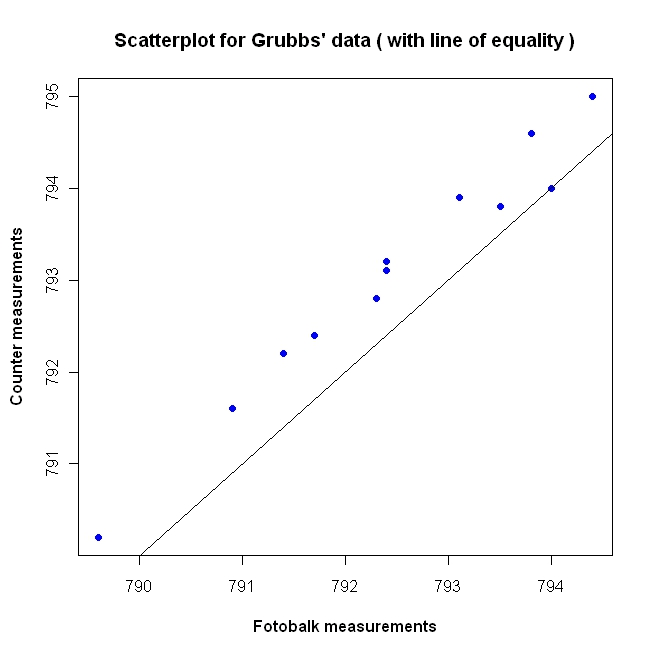
\includegraphics[width=100mm]{images/GrubbsScatter.jpeg}
			\caption{Scatter plot For Fotobalk and Counter Methods.}\label{GrubbsScatter}
		\end{center}
	\end{figure}
	
	\citet{Dewitte} notes that scatter plots were very seldom presented in the Annals of Clinical Biochemistry. This apparently
	results from the fact that the `Instructions for Authors' dissuade the use of regression analysis, which conventionally is accompanied by a scatter plot.
	

	\subsection{Bland-Altman plots}
	
	In light of shortcomings associated with scatterplots, \citet*{BA83} recommend a further analysis of the data. Firstly
	case-wise differences of measurements of two methods $d_{i} = y_{1i}-y_{2i} \mbox{ for }i=1,2,\dots,n$ on the same subject
	should be calculated, and then the average of those measurements ($a_{i} = (y_{1i} + y_{2i})/2 \mbox{ for }i=1,2,\dots, n$).
	
	\citet{BA83} proposes a scatterplot of the case-wise averages and differences of two methods of measurement. This scatterplot has since become widely known as the Bland-Altman plot. \citet*{BA83} express the
	motivation for this plot thusly:
	\begin{quote}
		``From this type of plot it is much easier to assess the magnitude
		of disagreement (both error and bias), spot outliers, and see
		whether there is any trend, for example an increase in (difference) for high values. This way of plotting the data is a very powerful way of displaying the results of a method comparison study."
	\end{quote}
	
	The case wise-averages capture several aspects of the data, such as expressing the range over which the values were taken, and assessing whether the assumptions of constant variance holds.
	Case-wise averages also allow the case-wise differences to be presented on a two-dimensional plot, with better data visualization qualities than a one dimensional plot. \citet{BA86}
	cautions that it would be the difference against either measurement value instead of their average, as the difference relates to both value. This methodology has proved very popular, and the Bland-Altman plots is widely regarded as powerful graphical methodology for making a visual assessment of the data.
	
	The magnitude of the inter-method bias between the two methods is simply the average of the differences $\bar{d}$. This inter-method bias is represented with a line on the Bland-Altman plot. As the objective of the Bland-Altman plot is to advise on the agreement of two methods, it is the case-wise differences that are also particularly relevant. The variances around this bias is estimated by the standard deviation of these differences $S_{d}$.
	
	\subsection{Bland-Altman plots for the Grubbs data}
	
	In the case of the Grubbs data the inter-method bias is $-0.61$ metres per second, and is indicated by the dashed line on Figure 1.2. By inspection of the plot, it is also possible to compare the precision of each method. Noticeably the differences tend to increase as the averages increase.
	
	
	The Bland-Altman plot for comparing the `Fotobalk' and `Counter'
	methods, which shall henceforth be referred to as the `F vs C' comparison,  is depicted in Figure 1.2, using data from Table 1.3.
	The presence and magnitude of the inter-method bias is indicated
	by the dashed line.
	\newpage
	
	%Later it will be shown that case-wise differences are the sole
	%component of the next part of the methodology, the limits of
	%agreement.
	
	
	\begin{table}[h!]
		\renewcommand\arraystretch{0.7}%
		\begin{center}
			\begin{tabular}{|c||c|c||c|c|}
				\hline
				Round & Fotobalk  & Counter  & Differences  & Averages  \\
				&  [F] & [C] & [F-C] &  [(F+C)/2] \\
				\hline
				1 & 793.8 & 794.6 & -0.8 & 794.2 \\
				2 & 793.1 & 793.9 & -0.8 & 793.5 \\
				3 & 792.4 & 793.2 & -0.8 & 792.8 \\
				4 & 794.0 & 794.0 & 0.0 & 794.0 \\
				5 & 791.4 & 792.2 & -0.8 & 791.8 \\
				6 & 792.4 & 793.1 & -0.7 & 792.8 \\
				7 & 791.7 & 792.4 & -0.7 & 792.0 \\
				8 & 792.3 & 792.8 & -0.5 & 792.5 \\
				9 & 789.6 & 790.2 & -0.6 & 789.9 \\
				10 & 794.4 & 795.0 & -0.6 & 794.7 \\
				11 & 790.9 & 791.6 & -0.7 & 791.2 \\
				12 & 793.5 & 793.8 & -0.3 & 793.6 \\
				\hline
			\end{tabular}
			\caption{Fotobalk and Counter methods: differences and averages.}
		\end{center}
	\end{table}
	
	\begin{table}[h!]
		\renewcommand\arraystretch{0.7}%
		\begin{center}
			\begin{tabular}{|c||c|c||c|c|}
				\hline
				Round & Fotobalk  & Terma  & Differences  & Averages  \\
				&  [F] & [T] & [F-T] &  [(F+T)/2] \\
				\hline
				1 & 793.8 & 793.2 & 0.6 & 793.5 \\
				2 & 793.1 & 793.3 & -0.2 & 793.2 \\
				3 & 792.4 & 792.6 & -0.2 & 792.5 \\
				4 & 794.0 & 793.8 & 0.2 & 793.9 \\
				5 & 791.4 & 791.6 & -0.2 & 791.5 \\
				6 & 792.4& 791.6 & 0.8 & 792.0 \\
				7 & 791.7 & 791.6 & 0.1 & 791.6 \\
				8 & 792.3 & 792.4 & -0.1 & 792.3 \\
				9 & 789.6 & 788.5 & 1.1 & 789.0 \\
				10 & 794.4 & 794.7 & -0.3 & 794.5 \\
				11 & 790.9 & 791.3 & -0.4 & 791.1 \\
				12 & 793.5 & 793.5 & 0.0 & 793.5 \\
				
				\hline
			\end{tabular}
			\caption{Fotobalk and Terma methods: differences and averages.}
		\end{center}
	\end{table}
	
	\newpage
	
	\begin{figure}[h!]
		\begin{center}
			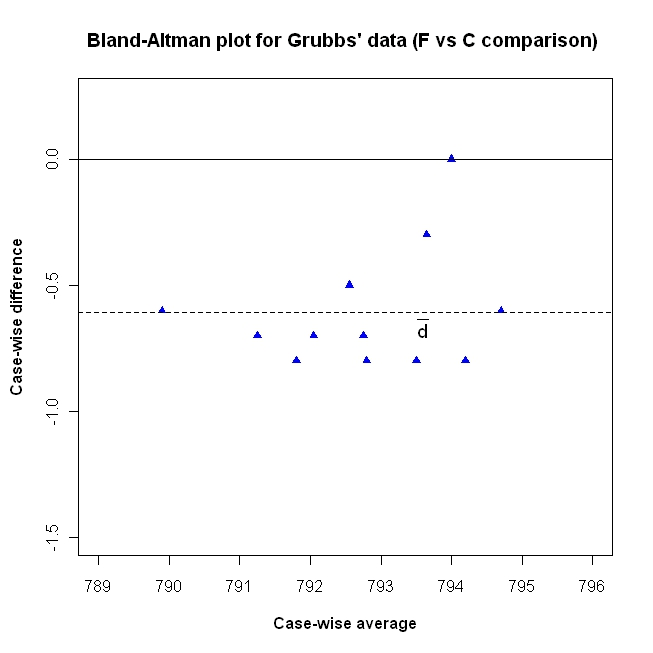
\includegraphics[width=120mm]{images/GrubbsBAplot-noLOA.jpeg}
			\caption{Bland-Altman plot For Fotobalk and Counter methods.}\label{GrubbsBA-noLOA}
		\end{center}
	\end{figure}
	
	
	
	In Figure 1.3 Bland-Altman plots for the `F vs C' and `F vs T'
	comparisons are shown, where `F vs T' refers to the comparison of
	the `Fotobalk' and `Terma' methods. Usage of the Bland-Altman plot
	can be demonstrate in the contrast between these comparisons. By inspection, there exists a larger inter-method bias in the `F vs C' comparison than in the `F vs T' comparison. Conversely there
	appears to be less precision in `F vs T' comparison, as indicated
	by the greater dispersion of covariates.
	
	\begin{figure}[h!]
		\begin{center}
			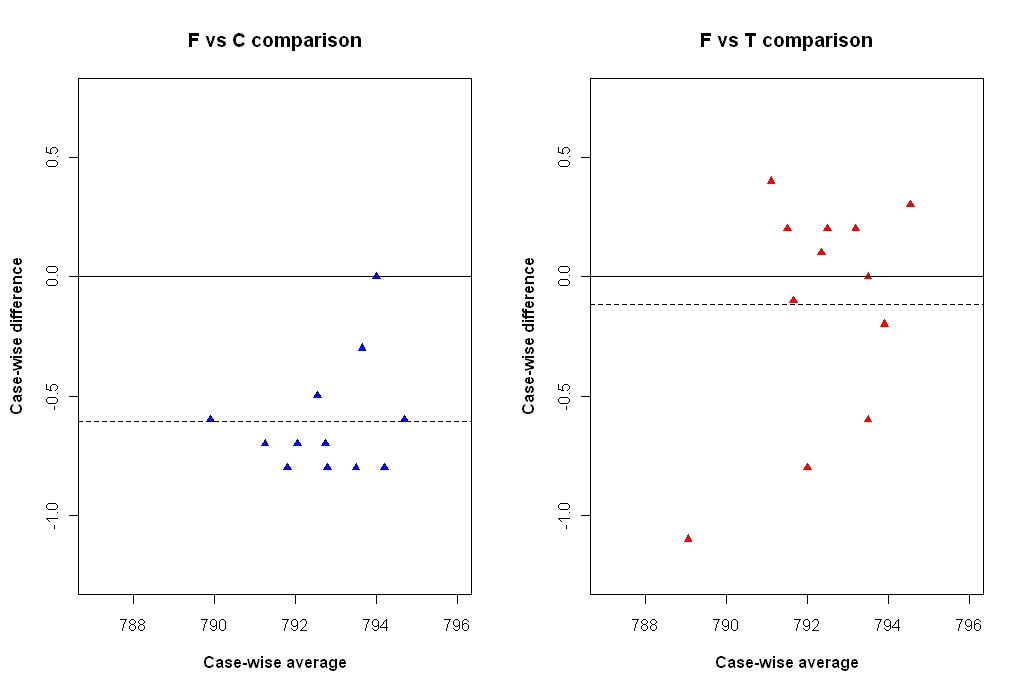
\includegraphics[height=90mm]{images/GrubbsDataTwoBAplots.jpeg}
			\caption{Bland-Altman plots for Grubbs' F vs C and F vs T comparisons.}\label{GrubbsDataTwoBAplots}
		\end{center}
	\end{figure}
	
	\newpage
	
	
	\subsection{Adverse features}
	
	Estimates for inter-method bias and variance of differences are only meaningful if there is uniform inter-bias and variability throughout the range of measurements. Fulfilment of these assumptions can be checked by visual inspection of the plot.The prototype Bland-Altman plots depicted in Figures 1.4, 1.5 and 1.6 are derived from simulated data, for the purpose of demonstrating how the plot would inform an analyst of features that would adversely affect use of the recommended methodology.
	
	Figure 1.4 demonstrates how the Bland-Altman plot would indicate
	increasing variance of differences over the measurement range.
	Fitted regression lines, for both the upper and lower half of the
	plot, has been added to indicate the trend. Figure 1.5 is an
	example of cases where the inter-method bias changes over the
	measurement range. This is known as proportional bias, and is
	defined by \citet{ludbrook97} as meaning that `one method gives values that are higher (or lower) than those from the other by an 	amount that is proportional to the level of the measured variable'. In both Figures 1.4 and 1.5, the assumptions necessary
	for further analysis using the limits of agreement are violated.
	
	Application of regression techniques to the Bland-Altman plot, and
	subsequent formal testing for the constant variability of
	differences is informative. The data set may be divided into two
	subsets, containing the observations wherein the difference values
	are less than and greater than the inter-method bias respectively.
	For both of these fits, hypothesis tests for the respective slopes
	can be performed. While both tests can be considered separately,
	multiple comparison procedures, such as the Benjamini-Hochberg
	\citep{BH} test, should be also be used.
	
	\begin{figure}[h!]
		\begin{center}
			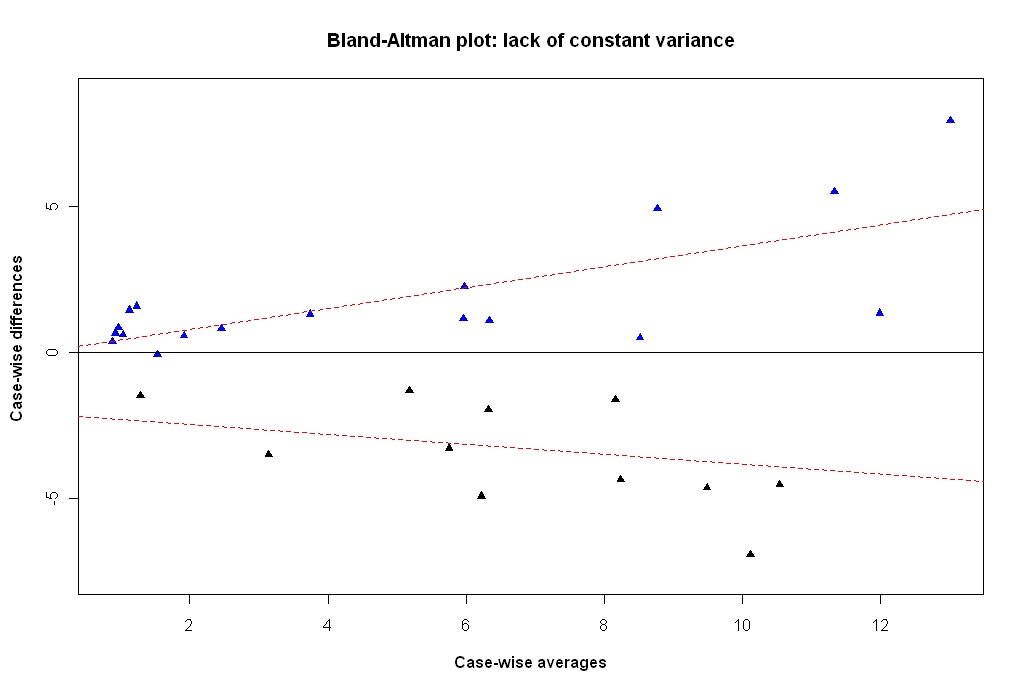
\includegraphics[height=90mm]{images/BAFanEffect.jpeg}
			\caption{Bland-Altman plot demonstrating the increase of variance over the range.}\label{BAFanEffect}
		\end{center}
	\end{figure}
	
	\begin{figure}[h!]
		\begin{center}
			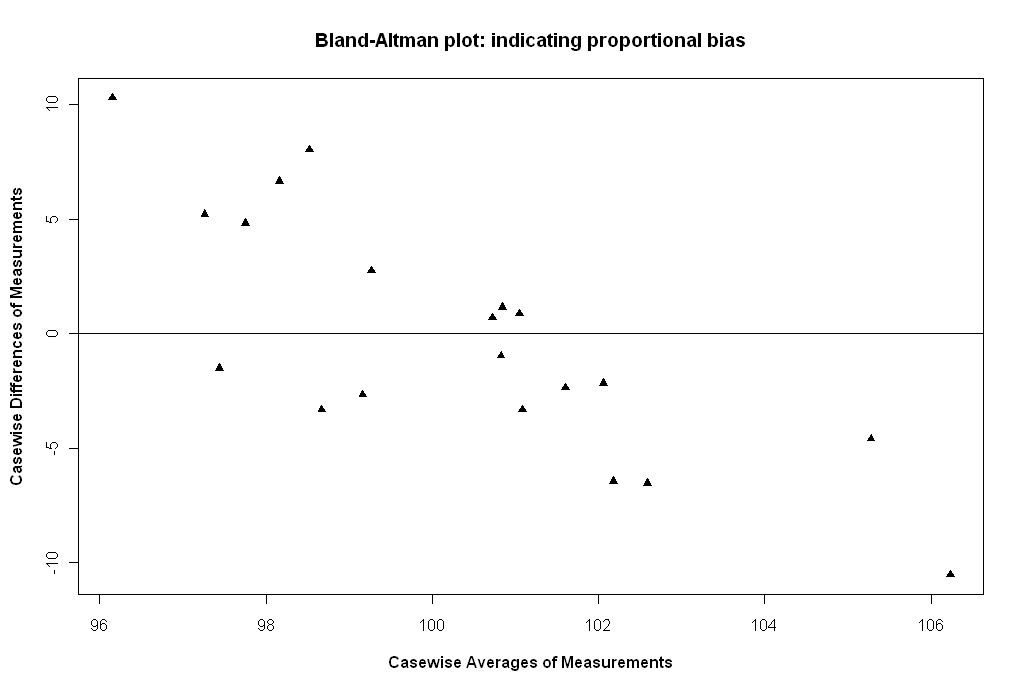
\includegraphics[height=90mm]{images/PropBias.jpeg}
			\caption{Bland-Altman plot indicating the presence of proportional bias.}\label{PropBias}
		\end{center}
	\end{figure}
	
	
	
	
	
	
	\subsection{Replicate Measurements}
	
	Thus far, the formulation for comparison of two measurement methods is one where one measurement by each method is taken on	each subject. Should there be two or more measurements by each methods, these measurement are known as `replicate measurements'.
	\citet{BXC2008} recommends the use of replicate measurements, but acknowledges the additional computational complexity.
	
	\citet*{BA86} address this problem by offering two different approaches. The premise of the first approach is that replicate
	measurements can be treated as independent measurements. The second approach is based upon using the mean of the each group of
	replicates as a representative value of that group. Using either
	of these approaches will allow an analyst to estimate the inter
	method bias.
	
	%\subsubsection{Mean of Replicates Limits of Agreement}
	
	However, because of the removal of the effects of the replicate
	measurements error, this would cause the estimation of the
	standard deviation of the differences to be unduly small.
	\citet*{BA86} propose a correction for this.
	
	\citet{BXC2008} takes issue with the limits of agreement based on
	mean values of replicate measurements, in that they can only be interpreted as prediction
	limits for difference between means of repeated measurements by
	both methods, as opposed to the difference of all measurements.
	Incorrect conclusions would be caused by such a misinterpretation.
	\citet{BXC2008} demonstrates how the limits of agreement
	calculated using the mean of replicates are `much too narrow as
	prediction limits for differences between future single
	measurements'. This paper also comments that, while treating the
	replicate measurements as independent will cause a downward bias
	on the limits of agreement calculation, this method is preferable
	to the `mean of replicates' approach.
	
	

\subsection{Sampling Protocols}
Dunn discusses the sampling protocols in depth. Consider a random sample of N specimens. A simple design is a  set of measurements on each specimen using each of the two methods, yield 2N measurments. Dunn remarks that such a design would not yield much in the way of information.
The criticism projected at the correlation coefficient is only valid if one is specifically interested in assessing “agreement”. However, it should be used as an exploratory tool in the first instance.
Exchangealility encompasses the qualities of similar precision.



	
%------------------------------------------------------------------------------------------------%
\subsection{MCS Research Notes}
The problem of comparing two methods of measurement is ubiquitous in scientific literature.
The use of  well-established methodologies, such as the paired t-test, correlation and regression approaches is criticised in Altman and Bland(1983).
In the Bland-Altman papers, the British Standards Institute emerge as the key authority on the definition of the Limits of agreement.
It is assumed that, in the absence of a specified probability, that the level is 95\%.

Bland and Altman proposed a simple graphical technique, plotting the case-wise differences against the case-wise means of the respective measurements.
The benefit of such an approach is the plot makes it easier to assess the magnitude of the disagreement (both error and bias), spot outliers, and see whether there is any trend.

%------------------------------------------------------------------------------------------------%

\subsection{Underlying Model}
The model underlying the Bland-Altman approach can be expressed as an LME model with heterogeneous variances.
\[y_{ij} = \beta_j + b_i  + \varepsilon_{ij}\]
The case-wise differences and case-wise means follow a bivariate normal distribution, with expected values and variances specified as [input equations].
%------------------------------------------------------------------------------------------------%
\subsection{Outlier detection}
Additionally, there is no clear guidance in any of the Bland-Altman papers on the treatment of outliers that may arise in a plot.
An example used in Bland-Altman 1986 identifies a “clear outlier”, where it is advised by the authors that “in practice, one could omit this subject”.
Bland and Altman 1999 recommend the computationally intensive approach of calculating the limits of agreement with, and then without, suspected outliers, in order to assess the impact on the results. However, they are clear that they do not recommend excluding outliers from analyses.

%------------------------------------------------------------------------------------------------%
\section{Westgard et Al}
% Good Paper
% http://www.clinchem.org/content/43/11/2039.long
Westgard et al. (1)(2)(3) outlined the basic principles for method comparison in a clear, easy to follow manual. They also introduced the concept of allowable analytical error and gave an overview of published performance criteria. They recommended that the estimated analytical imprecision and bias be compared with these performance criteria in method evaluation as well as in method comparison. Their approach made use of a scatter-plot and calculations based on regression lines, but with confidence limits and judgment of acceptability based on the criteria for allowable analytical error.

These principles of comparing analytical performance with performance criteria, however, have not been universally accepted, and recent publications have criticized the misuse of correlation coefficients (4) and overinterpretation of regression lines in method comparison (5)(6)(7). Bland and Altman (4) recommended the difference plot (or bias plot or residual plot) as an alternative approach for method comparison. On the abscissa they used the mean value of the methods to be compared, to avoid regression towards the mean, and on the ordinate they plotted the calculated difference between measurements by the two methods. They further estimated the mean and standard deviation of differences and displayed horizontal lines for the mean and for ±2 × the standard deviation. However, they missed the concept of a more objective criterion for acceptability. Recently, Hollis (5) has recommended difference plots as the only acceptable method for method comparison studies for publication in Annals of Clinical Biochemistry, but without specifying criteria for acceptability.

However, a few difference plots with evaluation of acceptability according to defined criteria have been published, e.g., in evaluation of estimated biological variation compared with analytical imprecision (8), and in external quality assessment of plasma proteins for the possibilities of sharing common reference intervals (9).

Maybe the scarcity of such publications is more a question of interpretation of the data by plotting than a strict choice between scatter-plot and difference plot, as discussed by Stöckl (10) recently. Investigators seem to rely too much on regression lines and r-values, without doing the equally important interpretation of the data points of the plot. This is becoming more and more disadvantageous with the increasing number of Reference Methods available for comparison with field methods, because in these cases, it is not a question of finding some relationships, but simply of judging the field method to be acceptable or not.

NCCLS has recently published guidelines for method comparison and bias estimation by using patients’ samples (11), where both scatter-plots and bias plots are advised. The document also recommends plotting of single determinations as mean values and stresses the need of visual inspection of data. Further, comparison with performance criteria is recommended, but these criteria are not specified and they are not used in the graphical interpretation. Recently, Houbouyan et al. (12) used ratio plots in their validation protocol of analytical hemostasis systems, where they used a preset, but arbitrarily chosen, acceptance limit of inaccuracy of 15%.

In the following, we will use the difference plot (or bias plot) in combination with simple statistics for the principal judgment of the identity or acceptability of a field method. The difference plot makes it easier to apply the concept; in principle, however, the same evaluations could be performed for a scatter-plot in relation to the line of identity (y = x).

The aim of this contribution is to pay attention to the hypothesis of identity and the concept of acceptable analytical quality in method comparison, especially when one of the methods is a Reference Method.
	
	



\section{Other Types of Studies}
\citet{lewis} categorize method comparison studies into three
different types.  The key difference between the first two is
whether or not a `gold standard' method is used. In situations
where one instrument or method is known to be `accurate and
precise', it is considered as the`gold standard' \citep{lewis}. A
method that is not considered to be a gold standard is referred to
as an `approximate method'. In calibration studies they are
referred to a criterion methods and test methods respectively.


\textbf{1. Calibration problems}. The purpose is to establish a
relationship between methods, one of which is an approximate
method, the other a gold standard. The results of the approximate
method can be mapped to a known probability distribution of the
results of the gold standard \citep{lewis}. (In such studies, the
gold standard method and corresponding approximate method are
generally referred to a criterion method and test method
respectively.) \citet*{BA83} make clear that their methodology is
not intended for calibration problems.

\bigskip \textbf{2. Comparison problems}. When two approximate
methods, that use the same units of measurement, are to be
compared. This is the case which the Bland-Altman methodology is
specfically intended for, and therefore it is the most relevant of
the three.



\bigskip \textbf{3. Conversion problems}. When two approximate
methods, that use different units of measurement, are to be
compared. This situation would arise when the measurement methods
use 'different proxies', i.e different mechanisms of measurement.
\citet{lewis} deals specifically with this issue. In the context
of this study, it is the least relevant of the three.
	%%%%%%%%%%%%%%%%%%%%%%%%%%%%%%%%%%%%%%%%%%%%%%%%%%%%%%%%%%%%%%%%%%%%%%%%%%%%%%%%%%%%%%%%%%%%%%%%%%%%%%%%

	\section{Fuzzy Gold Standards} The Gold Standard is considered to be the most
	accurate measurement of a particular parameter. But even gold
	standard raters must be assumed to have some level of measurement
	error. Fuzzy gold standard are considered by Phelps and Hutson (
	1994)
	
\citet[p.47]{DunnSEME} cautions that`gold standards' should not be
assumed to be error free. `It is of necessity a subjective
decision when we come to decide that a particular method or
instrument can be treated as if it was a gold standard'. The
clinician gold standard , the sphygmomanometer, is used as an
example thereof.  The sphygmomanometer `leaves considerable room
for improvement' \citep{DunnSEME}. \citet{pizzi} similarly
addresses the issue of glod standards, `well-established gold
standard may itself be imprecise or even unreliable'.


The NIST F1 Caesium fountain atomic clock is considered to be the
gold standard when measuring time, and is the primary time and
frequency standard for the United States. The NIST F1 is accurate
to within one second per 60 million years \citep{NIST}.

Measurements of the interior of the human body are, by definition,
invasive medical procedures. The design of method must balance the
need for accuracy of measurement with the well-being of the
patient. This will inevitably lead to the measurement error as
described by \citet{DunnSEME}. The magnetic resonance angiogram,
used to measure internal anatomy,  is considered to the gold
standard for measuring aortic dissection. Medical test based upon
the angiogram is reported to have a false positive reporting rate
of 5\% and a false negative reporting rate of 8\%. This is
reported as sensitivity of 95\% and a specificity of 92\%
\citep{ACR}.

In literature they are, perhaps more accurately, referred to as
`fuzzy gold standards' \citep{phelps}. Consequently when one of the methods is
essentially a fuzzy gold standard, as opposed to a `true' gold
standard, the comparison of the criterion and test methods should
be consider in the context of a comparison study, as well as of a
calibration study.


	
	
	
	\citet{DunnSEME} makes two important points in relation to these
	categories. Firstly he remarks that there isn't clear cut differences between each category.
	
	Secondly he comments on the clinician gold standard, the
	sphygmomanometer, \emph{leaves considerable room for improvement}.
	\citet{pizzi} also attends to this issue: \emph{well-established
		gold standard may itself be imprecise or even unreliable}.
	
	The Magnetic resonance angiogram is considered to the gold
	standard for measuring aortic dissection, with a sensitivity of
	95\% and a specificity of 92\% . \citep{ACR}
	
	In literature they are, perhaps more accurately, referred to as 'bronze standards'.
	
	Consequently when one of the methods is essentially a bronze
	standard, as opposed to a true gold standard, the comparison
	procedure should be considered as being of the second category.
	
	%============================================================ %
\newpage	\section{Fuzzball Agreement}
	Fuzzball agreement is a case where the correlation coefficient is close to zero. The sample values is restricted to a narrow range. but an examination of a relevant scatter-plot would indicate that
	there is agreement between the two methods.
	\\
	Agreement - a numerical measure Hutson et al define a numerical measure for agreement.
	\\
	For example, suppose the pairs of rater measurements are (1, 1), (1.1, 1), (1, 1.1), and (1.1, 1.1) then the sample Pearson correlation r = .0, yet the two raters or devices are considered to be in good agreement. We will refer to the instance where r is close to 0, yet there may be good agreement as "fuzzball agreement." \\Fuzzball agreement occurs quite often in practice when the sample values have very narrow or restricted ranges. Fuzzball agreement is just one instance where the correlation coefficient is a poor measure of agreement. \\Furthermore, note that the ICC is also a poor measure of agreement when there is fuzzball agreement. At the other extreme suppose the same raters given in the previous example had pairs of measurements (1, 101), (2, 102), (3, 103), and (4, 104) on the same relative scale as before. In this instance, r = 1.0, yet there is large disagreement between rater.
	

	\bigskip
\section{Repeatability and gold standards}
	Currently the phrase `gold standard' describes the most accurate method of measurement available. No other criteria are set out. Further to \citet{dunnSEME}, various gold standards have a varying levels of repeatability. Dunn cites the example of the sphygmomanometer, which is prone to measurement error. Consequently it can be said that a measurement method can be the `gold standard', yet have poor repeatability. Some authors, such as [cite] and [cite] have recognized this problem. Hence, if the most accurate method is considered to have poor repeatability, it is referred to as a 'bronze standard'.  Again, no formal definition of a 'bronze standard' exists.
	
	The coefficient of repeatability may provide the basis of formulation a formal definition of a `gold standard'. For example, by determining the ratio of $CR$ to the sample mean $\bar{X}$. Further to [Lin], it is preferable to have a sample size specified in advance. A gold standard may be defined as the method with the lowest value of $\lambda = CR /\bar{X}$ with $\lambda < 0.1\%$. Similarly, a silver standard may be defined as the method with the lowest value of $\lambda $ with $0.1\% \leq \lambda < 1\%$. Such thresholds are solely for expository purposes.
	
	\section{The Conversion Problem}

In this section, we will reconsider the conversion problem, where by the methods of measurements are denominated in different units.
Conversion problems arise when the comparison is between two 
approximate methods of measurement each of which measures the quantity in different units.

This situation can arise when the methods in question proceed by measuring different proxies for the underlying 
quantity of interest. (lewis 1991)

For the single measurement case, the author can not foresee any scope for insights that are not already offered by using a structural relation model, as proposed by lewis et 1991, or error-in-variables regression. 
In the case of orthonormal regression, it is not reasonable to assume that both methods have equal measurement variance, when they are denominated in different units.
The analyst may attempt to mitigate the problem by scaling the variance of one method, but even still problems remain.
Similarly for Deming regression, no further insights on how to properly estimate the variance ratio can be offered.

For the case of conversion problem with replicate measurements, a framework that incorporates the ideas offered by Roy (2009) can be proposed. Estimates for between-subject and within-subject variances may be sought.
However Roy's tests on variability are no longer applicable, as one would not expect the method to have similar estimates. An estimate for the scaling factor $\beta$ may be sought, where $Y_i \approx \beta X$.


\[ X_i = \tau_i + \delta_i \]
\[ Y_i = \alpha + \beta X \tau_i + \epsilon_i\]


We will simulate a data set based in lewis conversion problems, provide three replicates values for both measurements. To acheive this we add ``jitter noise" to three copies of each original measurement.

\addcontentsline{toc}{section}{Bibliography}

%--------------------------------------------------------------------------------------%

\bibliographystyle{chicago}
\bibliography{DB-txfrbib}
\end{document}

	
